\chapter{Progettazione}
\label{cap:progettazione}

\intro{Il seguente capitolo ha la funzione di illustrare l'architettura del sistema e i pattern utilizzati nel definirla.}

\setlength{\parskip}{3ex}

\section{Architettura}
Nella seguente sezione viene illustrato l'approccio iniziale e l'architettura del progetto commissionato.

\subsection{Approccio MDA}
La filosofia dell'azienda per fronteggiare nuove attività e progetti si basa su un approccio di tipo MDA (Model Driven Architecture). L'idea alla base di tale approccio risiede nel fatto che il cuore di ogni applicazione si traduce in un modello solido e ben strutturato. 

\setlength{\parskip}{3ex}

\noindent L'approccio MDA è stato utilizzato anche per affrontare la fase di progettazione del sistema commissionato. In particolare la prima attività è stata quella di definire i modelli su cui l'intero sistema si basa. Per modello si intende un oggetto che deve essere mappato e gestito in una opportuna tabella di un database relazionale.   

\pagebreak

\noindent In particolare i modelli identificati in base alle richieste del committente sono i seguenti:
\begin{itemize}
\item \textbf{Progetto} (Long idProponente, Long idReferente, String codice, String titolo, String descrizione, String statoAvanzamento, Integer giorni, Integer percentualeAvanzamento, GregorianCalendar dataInizio)

\setlength{\parskip}{3ex}

\noindent \textbf{DESCRIZIONE}: questo modello rappresenta un progetto commissionato all'azienda da parte di un cliente o ideato dall'azienda per raggiungere nuovi clienti.

\setlength{\parskip}{3ex}

\noindent \textbf{ATTRIBUTI}:
\begin{itemize}
\item \textit{idProponente} corrisponde all'identificativo del  proponente, ovvero l'azienda da cui nasce l'idea del progetto (CWBI o altro cliente);
\item \textit{idReferente} corrisponde all'identificativo di un dipendente di CWBI che assume il ruolo di responsabile del progetto;
\item \textit{codice} corrisponde ad un identificativo del progetti (es. 2023.70);
\item \textit{titolo} corrisponde al titolo del progetto;
\item \textit{descrizione} corrisponde alla descrizione generale  progetto che illustra l'obiettivo e le funzionalità;
\item \textit{statoAvanzamento} corrisponde allo stato attuale  del progetto. Lo stato può assumere i seguenti valori: {aperto, chiuso, approvato, rifiutato, sospeso};
\item \textit{giorni} corrisponde ai giorni di sviluppo previsti per portare a termine il progetto;
\item \textit{percentualeAvanzamento} corrisponde alla percentuale di avanzamento delle attività di progetto;
\item \textit{dataInizio} corrisponde alla data di inizio delle attività di progetto.
\end{itemize}

\setlength{\parskip}{6ex}

\item \textbf{CorrelazioneProgettoCliente} (Long idCliente, Long idProgettoCliente)

\setlength{\parskip}{3ex}

\textbf{DESCRIZIONE}: questo modello rappresenta la correlazione che persiste tra un progetto e un certo cliente. Si fa notare che uno stesso progetto può raggiungere più di un cliente.

\setlength{\parskip}{3ex}

\textbf{ATTRIBUTI}:
\begin{itemize}
\item \textit{idCliente} corrisponde all'identificativo di un cliente;
\item \textit{idProgettoCliente} corrisponde all'identificativo di un progetto esistente.
\end{itemize}

\pagebreak

\item \textbf{Offerta} (Long idCliente, Long idProgetto, String titolo, String descrizione, String stato, GregorianCalendar dataStipula, BigDecimal imponibile1, BigDecimal imponibile2, BigDecimal imponibile3)

\setlength{\parskip}{3ex}

\textbf{DESCRIZIONE}: questo modello rappresenta l'offerta che viene stipulata per un certo cliente in merito ad uno dei progetti a disposizione.

\setlength{\parskip}{3ex}

\textbf{ATTRIBUTI}:
\begin{itemize}
\item \textit{idCliente} corrisponde all'identificativo di un cliente;
\item \textit{idProgettoCliente} corrisponde all'identificativo di un progetto esistente;
\item \textit{titolo} corrisponde al titolo dell'offerta (es. Contratto n.7/2023);
\item \textit{descrizione} corrisponde alla descrizione dell'offerta emessa (note, informazioni utili, ecc.);
\textit{stato} corrisponde allo stato attuale dell'offerta. Lo stato può assumere i seguenti valori: in preparazione, in accettazione, accettata;
\item \textit{dataStipula} corrisponde alla data in cui l'offerta è stata emessa;
\item \textit{imponibile1} corrisponde al primo prezzo proposto per firmare l'offerta;
\item \textit{imponibile2} corrisponde al secondo prezzo proposto per firmare l'offerta;
\item \textit{imponibile3} corrisponde al terzo prezzo proposto per firmare l'offerta.
\end{itemize}
\end{itemize}

\setlength{\parskip}{6ex}

\noindent I modelli \textbf{Cliente} e \textbf{Utente}, necessari per realizzare il progetto commissionato, erano già stati definiti per un altro modulo dell'applicazione CW GEST. In particolare questi modelli presentano rispettivamente un cliente e un dipendente di CWBI. Dato che tali modelli presentano le medesime caratteristiche pensate per il progetto in questione non si è reso necessario alterarli per l'utilizzo.

\pagebreak

\subsection{Architettura MVC}
Come citato in precedenza, il framework Apache Struts mette a disposizione un'architettura MVC per costruire applicazioni web. In particolare l'architettura risulta essere la seguente:

\begin{figure}[!h]
	\centering
	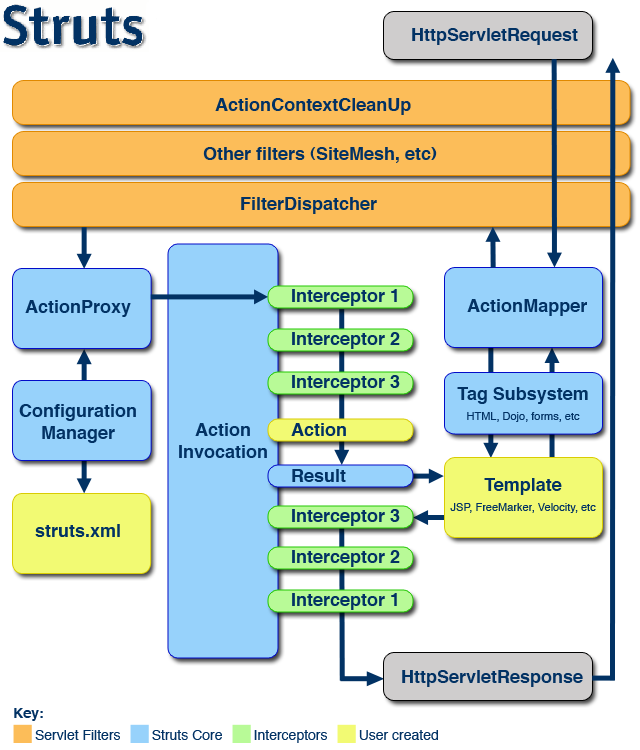
\includegraphics[width=9cm]{../images/MVC.png}
	\caption{Architettura MVC di Apache Struts}
\end{figure}

\section{Design pattern}
\subsection{Pattern IoC}


\subsection{Pattern DAO}
